\subsubsection{Procedure}

\begin{enumerate}
    \item populate store with dummy data (use same data from baseline benchmark)
    \item load 1 out of 4 pre-generated workloads (set of 1000 transactions with varying length working on varying data)
    \item distribute workload on pre-defined number of cores (1000 / num\_threads + amortization of remainder)
    \item fork threads with partial workloads
    \item each thread runs its transactions on the dummy data (repeats up to 3 times on failure, does not count tx if 4 attempts failed)
    \item measure time between fork and join (because timers on different cores are not synchronous)
    \item determine transaction throughput = num\_committed\_transactions / total\_time
    \item repeat this process 10 times for each workload (each workload is tied to a certain database size)
    \item after ten times: compute tx throughput, throughput speed up, parallel efficiency, and abort rate
\end{enumerate}

\paragraph{Types of Transactions}

\begin{itemize}
    \item short: between 2 and 32 operations
    \item long: between 64 and 256 operations
\end{itemize}

\paragraph{Probabilistic Distribution of Operations}

According to \cite{andrei2017sap}

\begin{itemize}
    \item READ: 84\%
    \item UPDATE: 16\% (including INSERT and DELETE)
\end{itemize}

\paragraph{Scenarios}

\begin{itemize}
    \item A: small database + short transactions (high contention, worst-case)
    \item B: small database + long transactions (very high contention, absolute worst-case)
    \item C: large database + short transactions (low contention)
    \item D: large database + long transactions (medium contention)
\end{itemize}

\paragraph{Metrics}

\begin{itemize}
    \item raw transaction throughput (no proper plot yet)
    \item speedup
    \item parallel efficiency
    \item abort rate
\end{itemize}

\subsubsection{Results}

\todo[inline]{The plots are already there (see below)}

\begin{figure}
\begin{minipage}[l]{0.50\textwidth}
        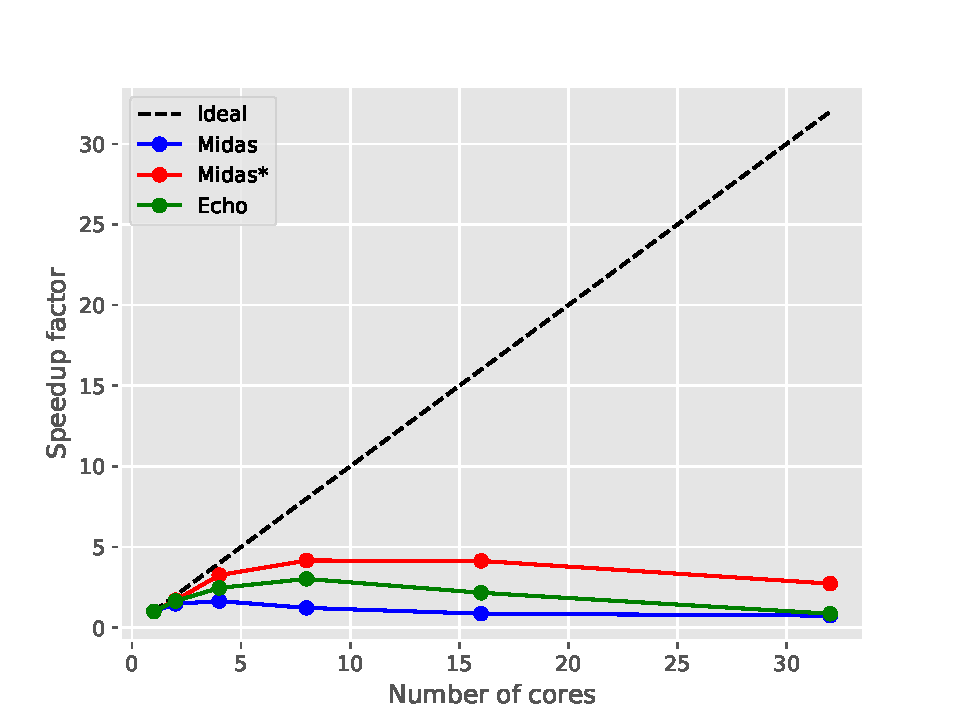
\includegraphics[width=\textwidth]{figures/bench/spd-ss}
        \caption{Transaction throughput speedup for scenario A}
        % \label{fig:concept-two-level-store}
\end{minipage}
\begin{minipage}[l]{0.50\textwidth}
    % \begin{figure}
        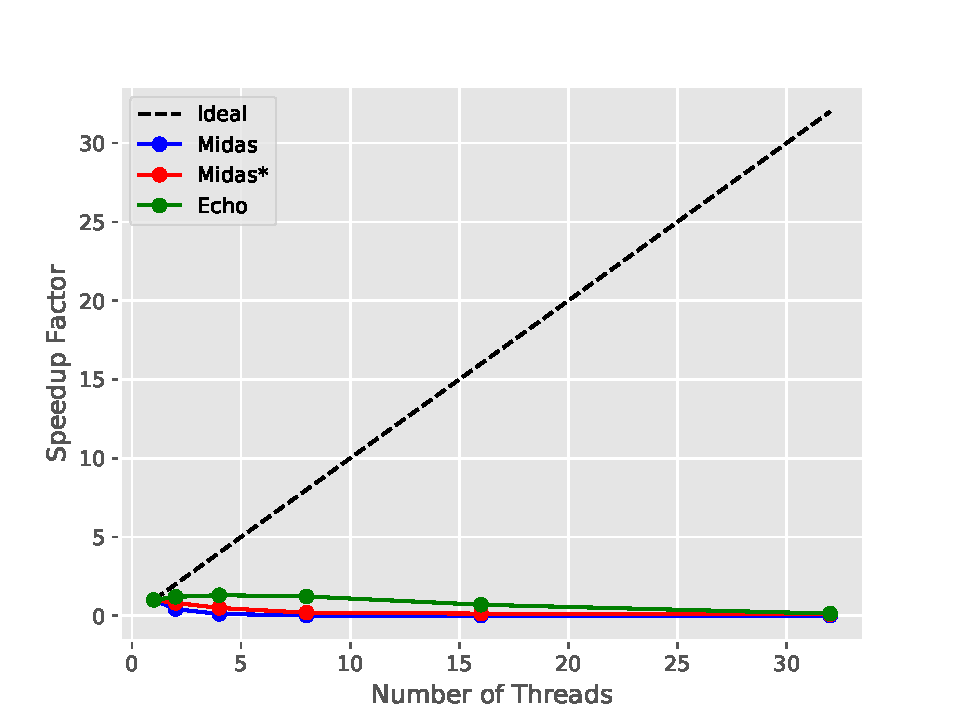
\includegraphics[width=\textwidth]{figures/bench/spd-sl}
        \caption{Transaction throughput speedup for scenario B}
        % \label{fig:concept-two-level-store}
    % \end{figure}
\end{minipage}
% \end{figure}

% \begin{figure}
\begin{minipage}[l]{0.50\textwidth}
        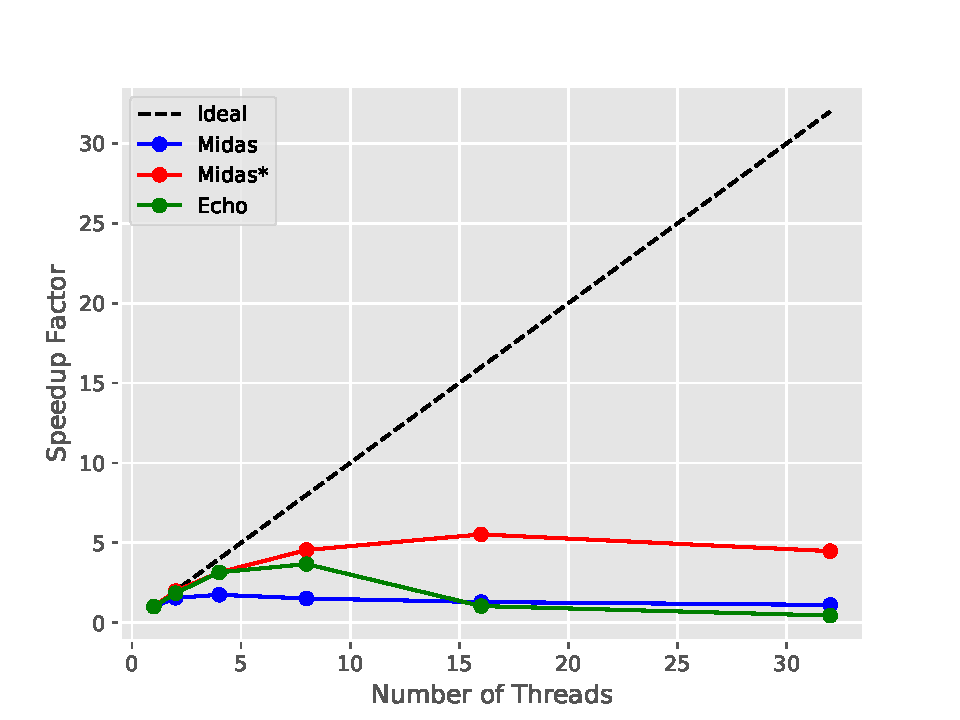
\includegraphics[width=\textwidth]{figures/bench/spd-ls}
        \caption{Transaction throughput speedup for scenario C}
        % \label{fig:concept-two-level-store}
    % \end{figure}
\end{minipage}
\begin{minipage}[l]{0.50\textwidth}
    % \begin{figure}
        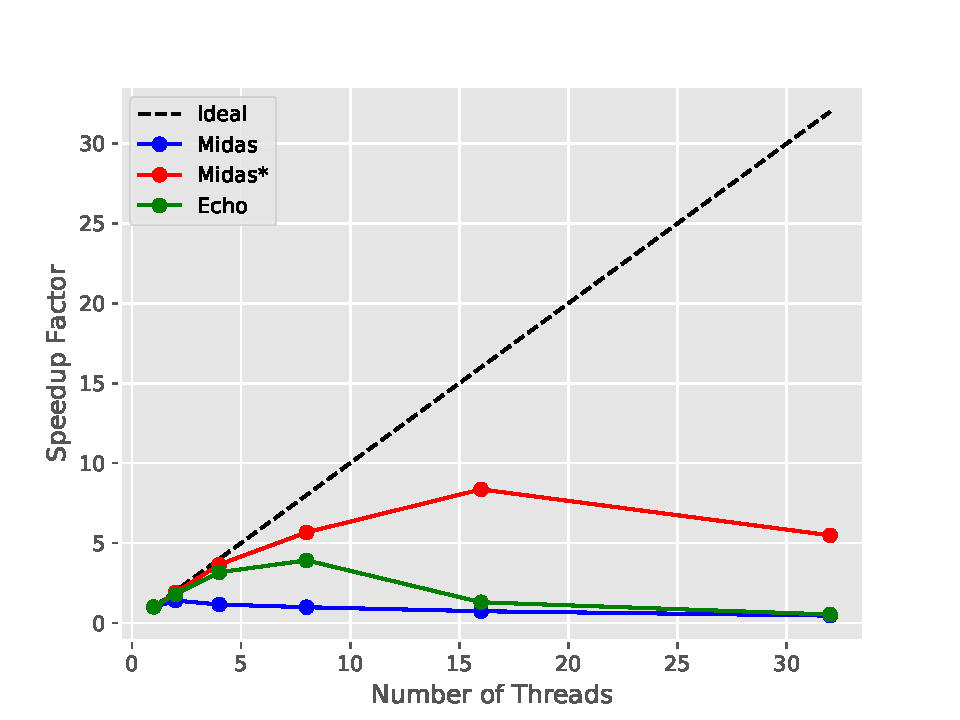
\includegraphics[width=\textwidth]{figures/bench/spd-ll}
        \caption{Transaction throughput speedup for scenario D}
        % \label{fig:concept-two-level-store}
\end{minipage}
\end{figure}

%==============================================================================
%==============================================================================
%==============================================================================

\begin{figure}
\begin{minipage}[l]{0.50\textwidth}
        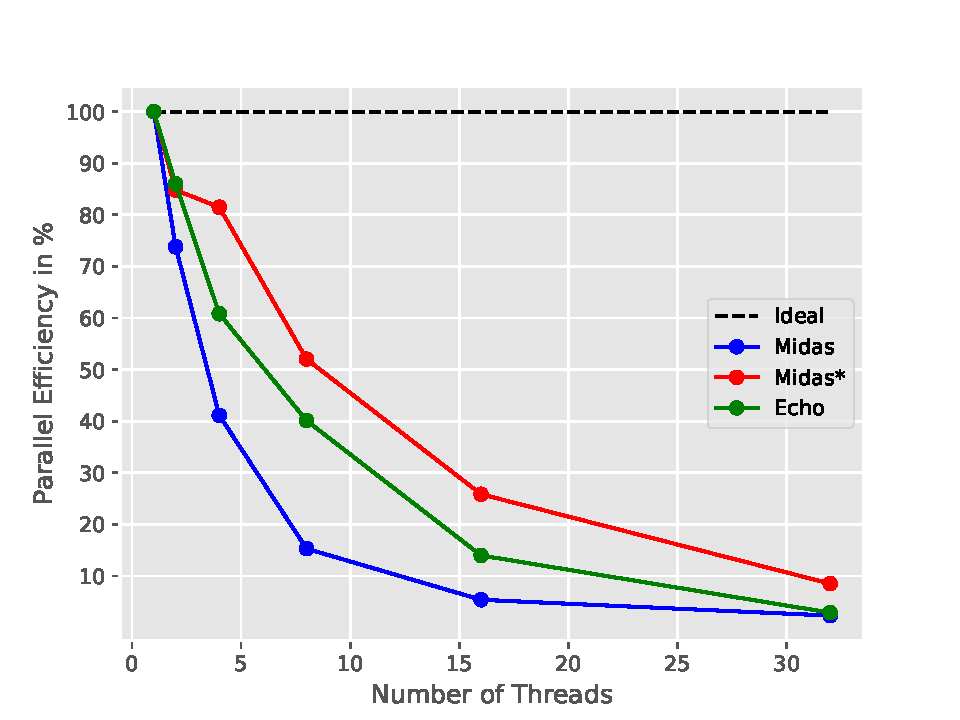
\includegraphics[width=\textwidth]{figures/bench/eff-ss}
        \caption{Parallel efficiency for scenario A}
        % \label{fig:concept-two-level-store}
\end{minipage}
\begin{minipage}[l]{0.50\textwidth}
    % \begin{figure}
        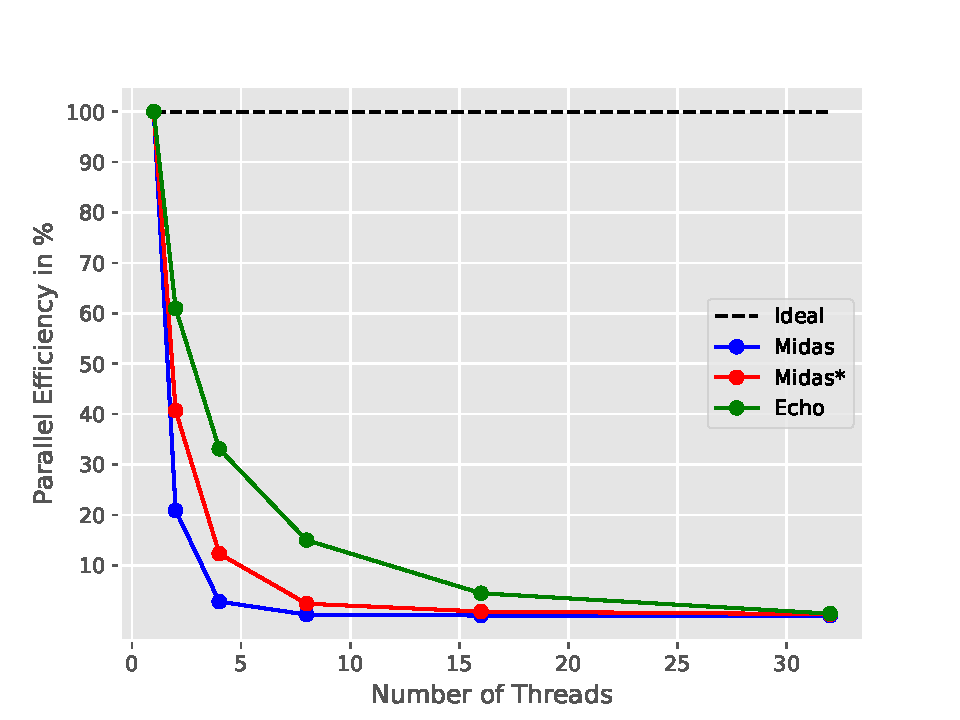
\includegraphics[width=\textwidth]{figures/bench/eff-sl}
        \caption{Parallel efficiency for scenario B}
        % \label{fig:concept-two-level-store}
    % \end{figure}
\end{minipage}
% \end{figure}

% \begin{figure}
\begin{minipage}[l]{0.50\textwidth}
        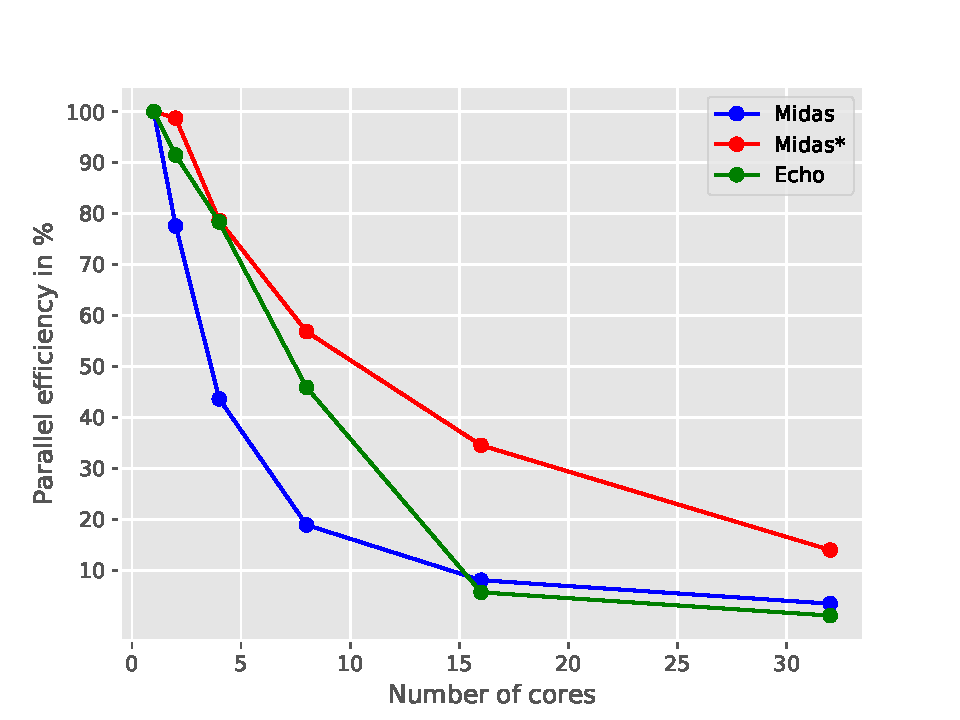
\includegraphics[width=\textwidth]{figures/bench/eff-ls}
        \caption{Parallel efficiency for scenario C}
        % \label{fig:concept-two-level-store}
    % \end{figure}
\end{minipage}
\begin{minipage}[l]{0.50\textwidth}
    % \begin{figure}
        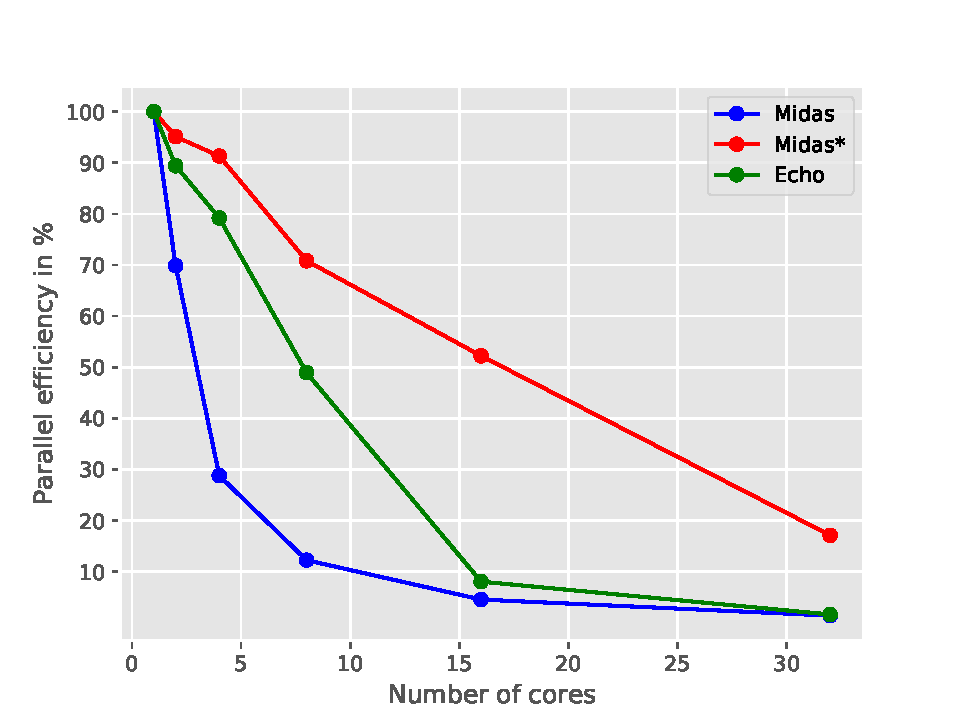
\includegraphics[width=\textwidth]{figures/bench/eff-ll}
        \caption{Parallel efficiency for scenario D}
        % \label{fig:concept-two-level-store}
\end{minipage}
\end{figure}

%==============================================================================
%==============================================================================
%==============================================================================

\begin{figure}
\begin{minipage}[l]{0.50\textwidth}
        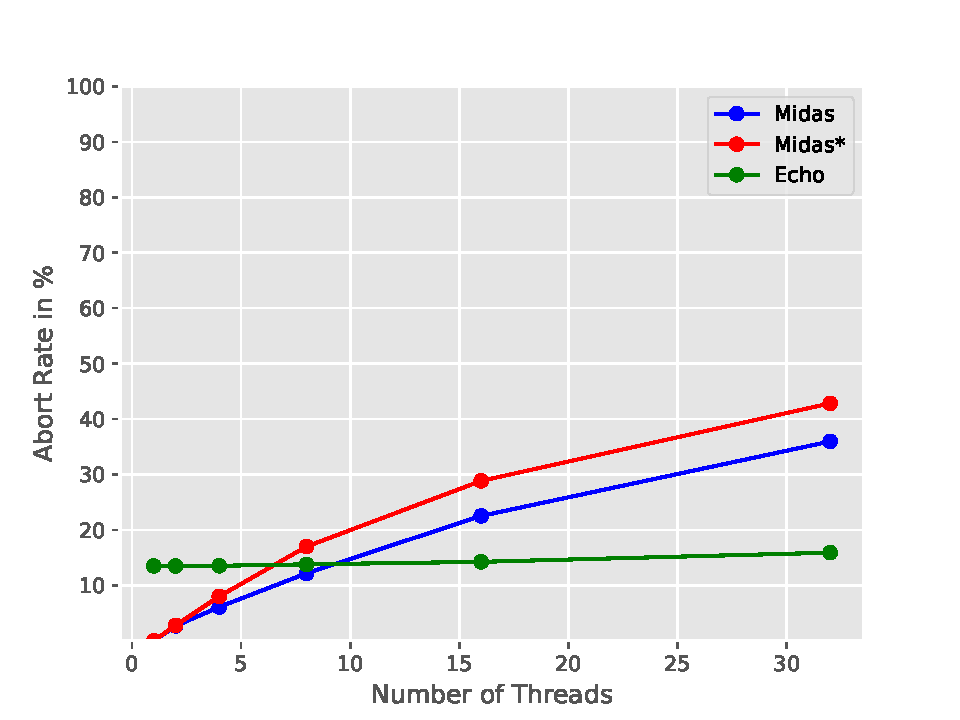
\includegraphics[width=\textwidth]{figures/bench/ar-ss}
        \caption{Abort rates for scenario A}
        % \label{fig:concept-two-level-store}
\end{minipage}
\begin{minipage}[l]{0.50\textwidth}
    % \begin{figure}
        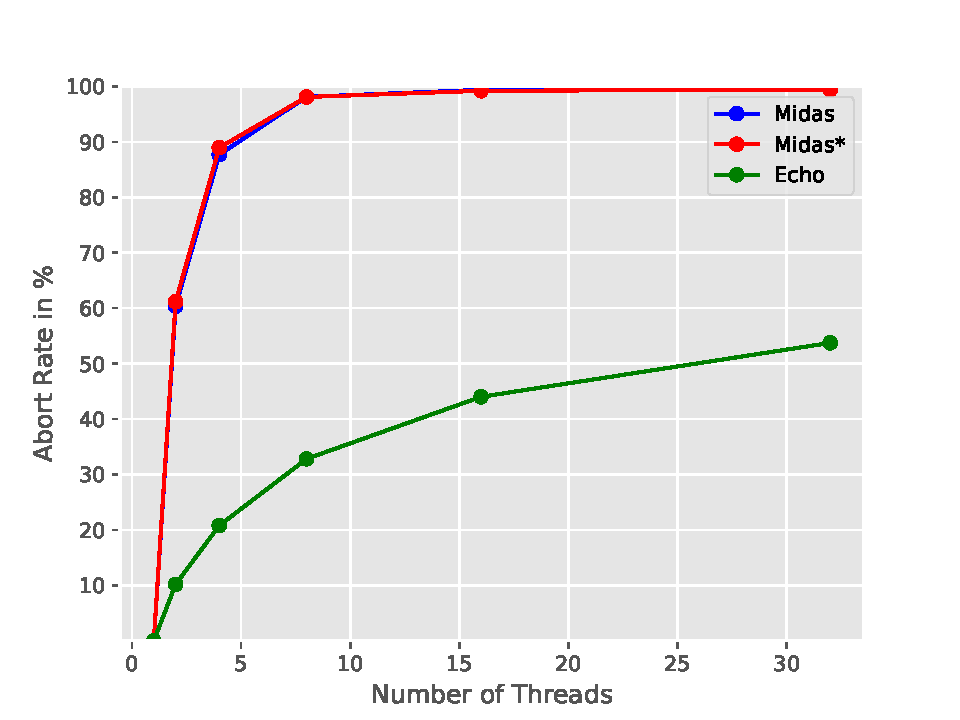
\includegraphics[width=\textwidth]{figures/bench/ar-sl}
        \caption{Abort rates for scenario B}
        % \label{fig:concept-two-level-store}
    % \end{figure}
\end{minipage}
% \end{figure}

% \begin{figure}
\begin{minipage}[l]{0.50\textwidth}
        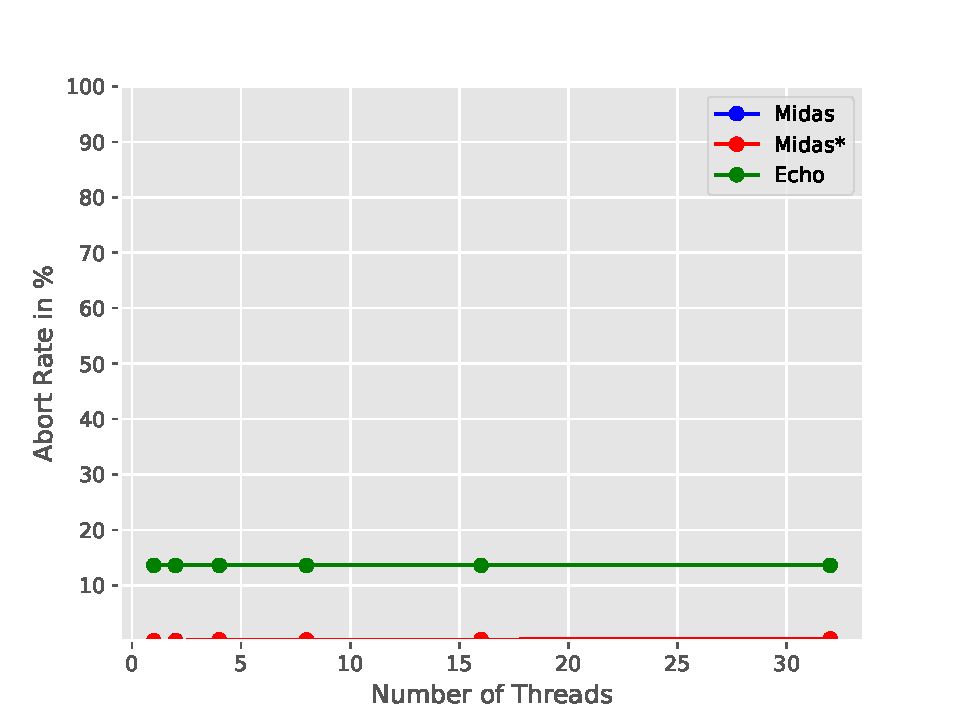
\includegraphics[width=\textwidth]{figures/bench/ar-ls}
        \caption{Abort rates for scenario C}
        % \label{fig:concept-two-level-store}
    % \end{figure}
\end{minipage}
\begin{minipage}[l]{0.50\textwidth}
    % \begin{figure}
        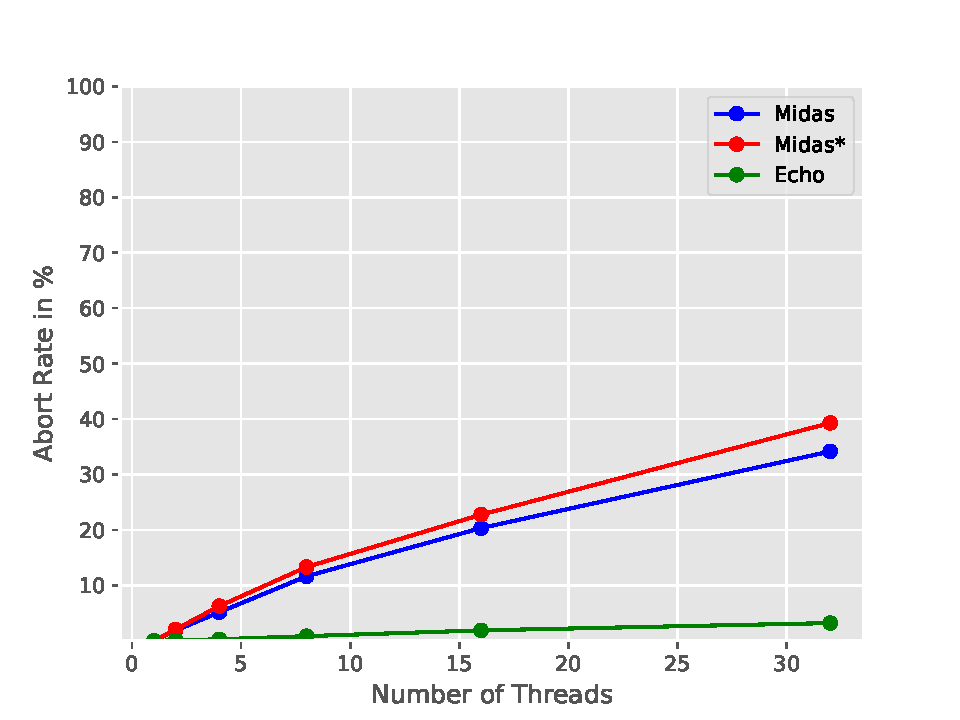
\includegraphics[width=\textwidth]{figures/bench/ar-ll}
        \caption{Abort rates for scenario D}
        % \label{fig:concept-two-level-store}
\end{minipage}
\end{figure}

\subsubsection{Discussion}

\todo[inline]{discuss results}
